\documentclass{article}
\usepackage[pdfcreator={LaTeX}]{hyperref}
\usepackage{graphicx}
\usepackage[utf8]{inputenc} 
\usepackage[ngerman]{babel}


\usepackage{tikz}
\usetikzlibrary{arrows,shadows}
\usepackage{pgf-umlsd}


\begin{document}
\begin{titlepage}

\begin{center}
\textbf{\textsc{\LARGE Spezifikation}}

{\large \today}

\vspace{2cm}
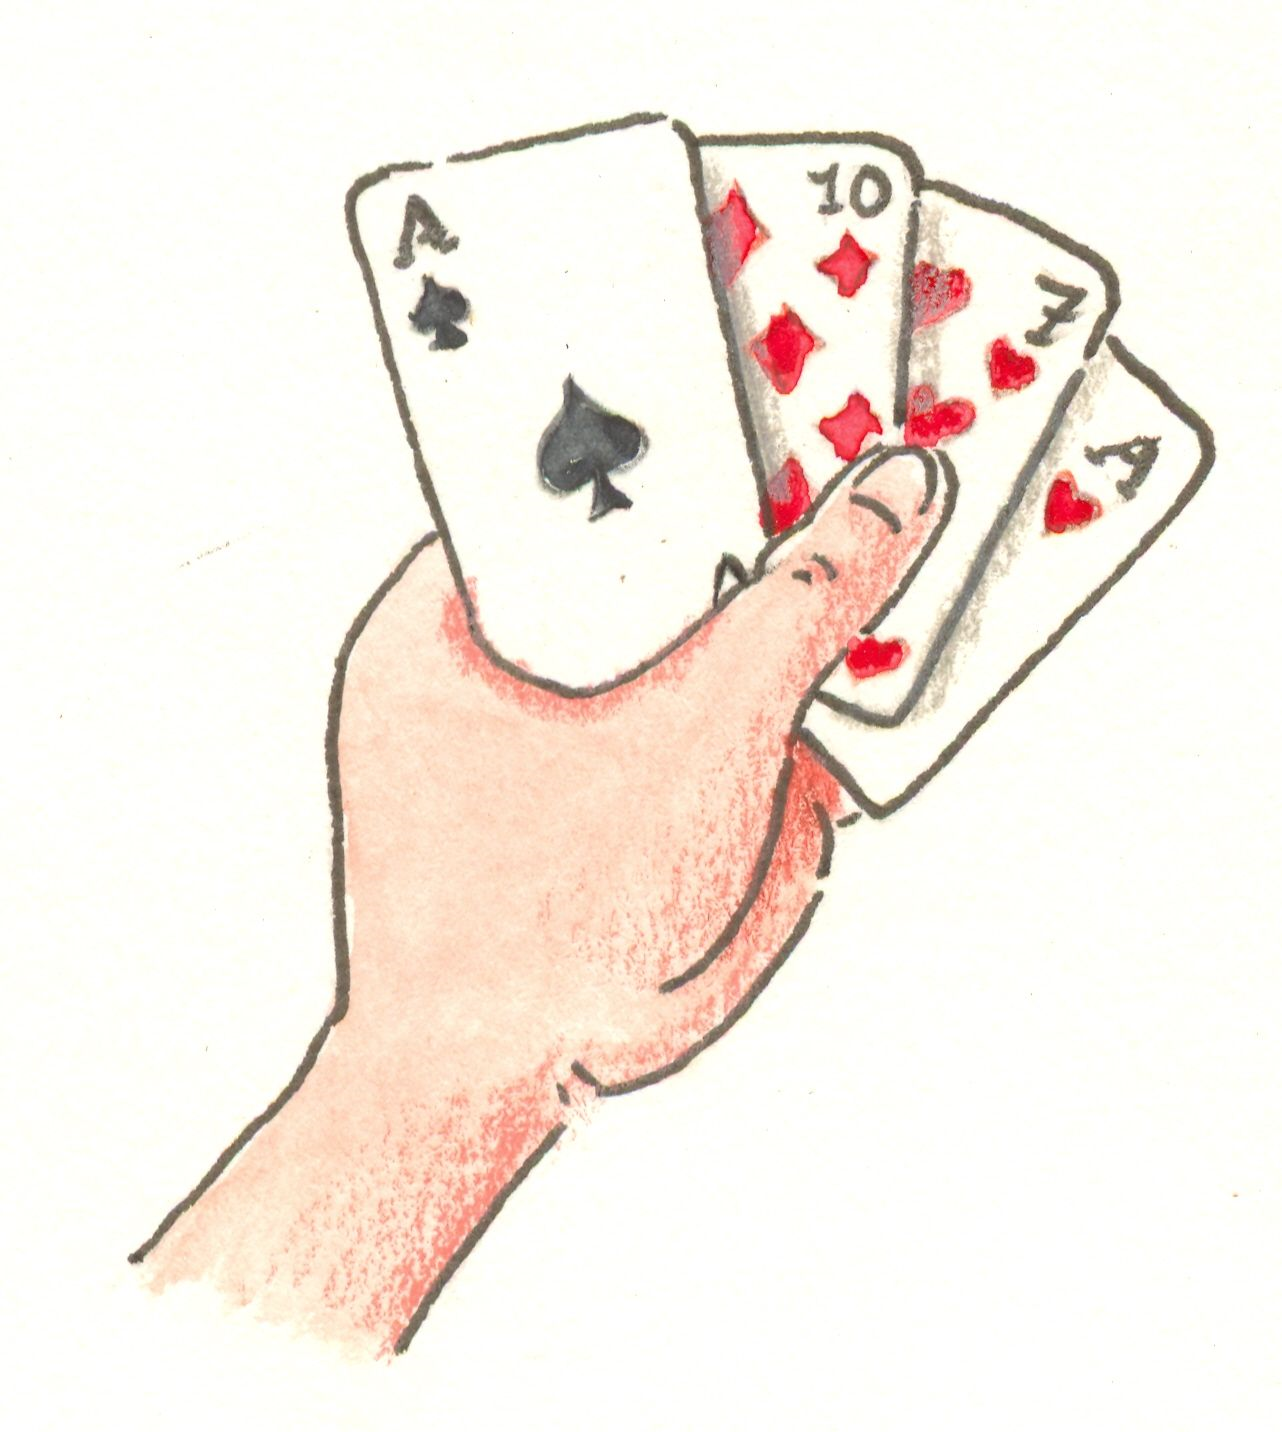
\includegraphics{kartenspiel}
\ \\
\ \\

\textbf{\textsc{\LARGE NET-WizHearts}}
\vspace{2cm}

\begin{tabular}{|c|c|c|}\hline
   Phase & Verantwortlicher & E-Mail \\ \hline\hline
   Pflichtenheft & Alina Meixl &  alina@meixl.de \\ \hline
   Entwurf & Viktoria Witka & witkaviktoria@freenet.de \\ \hline
   Spezifikation & Daniel Riedl & dariedl14@yahoo.de \\ \hline
   Implementation & Andreas Altenbuchner& a.andi007@gmail.com\\ \hline
   Verifikation & Patrick Kubin & kubin@fim.uni-passau.de\\ \hline
   Präsentation & w& w\\ \hline
 \end{tabular}

\end{center}

\end{titlepage}

\tableofcontents
\newpage

\section{Einleitung}
Hier kommt die Spezifikation.
\  \\


\section{Systemarchitektur}
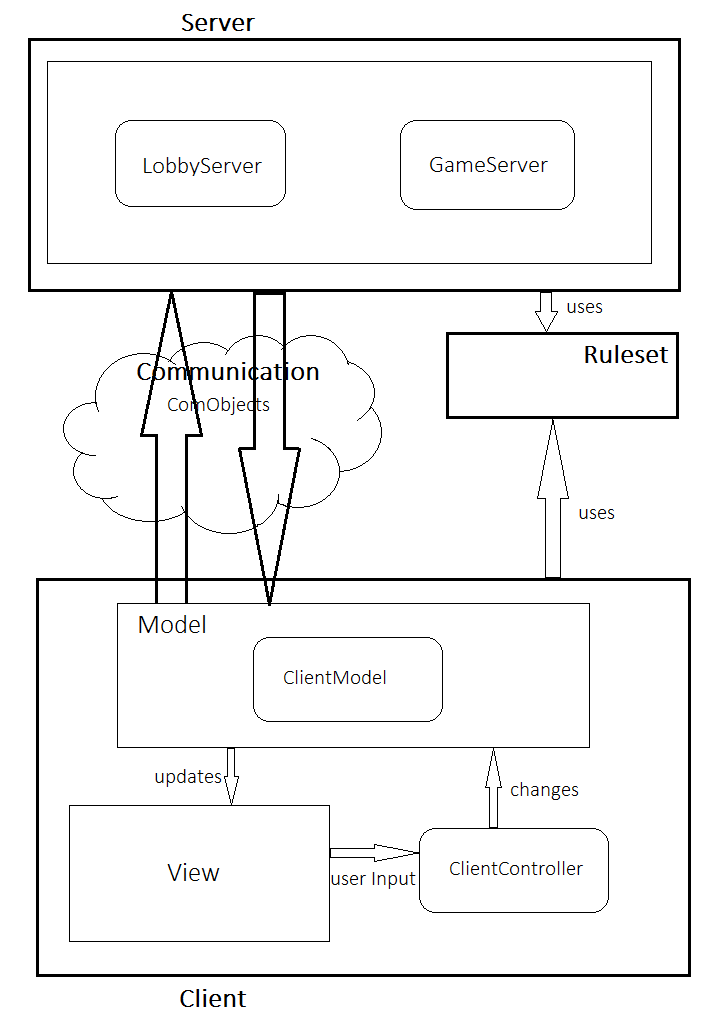
\includegraphics[width=\textwidth]{ArchitekturDiagramm}
\newpage

\section{Klassendiagramm}

\subsection{Packages}
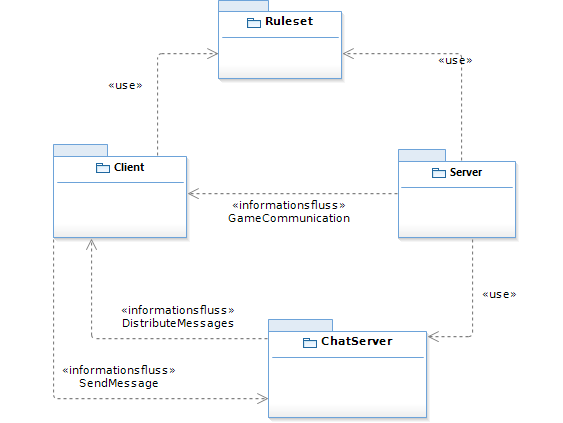
\includegraphics[width=\textwidth]{Packages}
\newpage

\section{Änderungen am Entwurf}
\subsection{Zusätzliche Pattern}
\subsubsection{Factory Pattern}
Objekte erstellen, Messages
\subsubsection{Builder Pattern}
Zum zeichnen der Karten
\subsubsection{Visitor Pattern}
...

\subsection{Server}
Der Server war zuletzt ein Interface. Wir haben uns dennoch entschieden die Serverklasse als abstrakte Klasse zu schreiben. So können die Methoden an die 'unteren' Server vererbt werden und wenn nötig überschrieben. Auch die Aggregagtion stimmt somit wieder.
\subsection{}
\subsection{}
\subsection{}
\subsection{}
\newpage

\section{Spezifizierung der Klassen}
\subsection{Client}
Methoden
Attribute
Beschreibung

Gespeichterte Daten?? für Karten
\subsubsection{ClientMain}
\subsubsection{ClientController}
\subsubsection{ClientModel}
\subsubsection{MessageListenerThread}
\subsubsection{MVMessage}
\subsubsection{MVLobby}
\subsubsection{MVGameLobby}
\subsubsection{MVGame}
\subsubsection{Window}
\subsubsection{WizID}
\subsubsection{HeartsID}
\newpage

\subsection{View}
\subsubsection{Lobby}
\subsubsection{GameLobby}
\subsubsection{Game}
\subsubsection{Password}
\subsubsection{CreateGame}
\subsubsection{Login}
\subsubsection{ChooseItem}
\subsubsection{Warning}
\subsubsection{InputNumber}
\subsubsection{MVMessages}
\subsubsection{ScoreWindow}
\subsubsection{ChooseCards}
\subsubsection{GamePanel}
\subsubsection{DiscardPile}
\subsubsection{DrawDesk}
\subsubsection{OtherPlayer}
\subsubsection{OwnHand}
\subsubsection{Language}
\newpage

\subsection{Ruleset}
\subsubsection{ServerRuleset}
\subsubsection{Wizard}
\subsubsection{Hearts}
\subsubsection{GameState}
\subsubsection{GameClientUpdate}
\subsubsection{HeartsData}
\subsubsection{WizData}
\subsubsection{PlayerState}
\subsubsection{Card}
\subsubsection{OtherData}
\subsubsection{GamePhase}
\subsubsection{WizardCard}
\subsubsection{HeartsCard}
\newpage

\subsection{Server}
\subsubsection{ServerMain}
\subsubsection{LobbyServer}
\subsubsection{GameServer}
\subsubsection{ClientListenerThread}
\subsubsection{GameServer}
\subsubsection{Server}
\subsubsection{Player}
\subsubsection{GameServerRepräsentation}
\newpage

\subsection{ComObjects}
\subsubsection{Ruleset}
\subsubsection{ComObject}
\subsubsection{Commands}
\subsubsection{ComLogin}
\subsubsection{ComUpdatePlayerlist}
\subsubsection{ComInitGameLobby}
\subsubsection{ComChatMessage}
\subsubsection{ComPassword}
\subsubsection{ComJoinRequest}
\subsubsection{ComKicklayer}
\subsubsection{ComInitGameLobby}
\subsubsection{ComLobbyUpdateGamelist}
\newpage

\section{JUnit-Tests}
\newpage

\section{Implementierungsplan}
\subsection{Arbeitspakete}
\includegraphics[scale=0.9]{Arbeitspakete}
\subsection{Gantt-Diagramm}
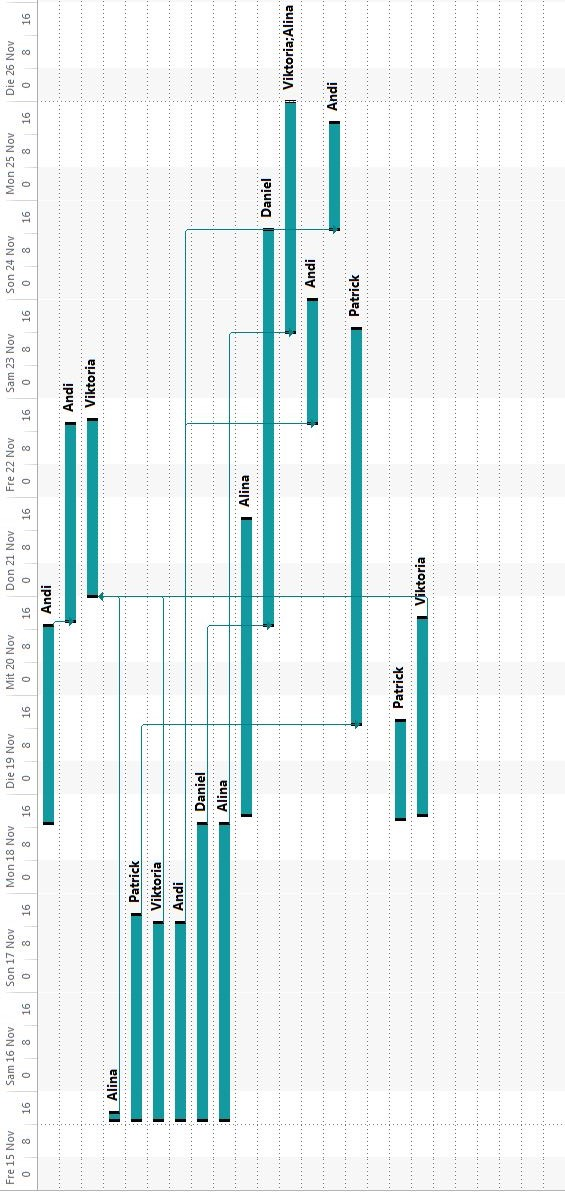
\includegraphics[scale=0.7]{Gantt}

\end{document}
